\subsubsection{Deauthentication Denial of Service}
\label{ddos-atk}
The deauthentication denial of service (DOS) \cite{research:disassoc_atk} is a complex attack that takes advantage of the unencrypted nature of the management frames by spoofing disassociation or deauthentication frames, depending on whether the attacker wants to block a single device or all devices from the network. It is a denial of service attack that targets the MAC layer in the TCP/IP Model pictured in figure \ref{tcpip}, there are other attacks designed for the other layers \cite{research:layer_flood}.

When a client wishes to gracefully disconnect from a 802.11 network it sends a disassociation frame \cite{research:80211_disassoc_frame} to the access point, likewise when an AP needs to disconnect from a client it sends a deauthentication \cite{research:80211_deauth_frame} frame. If the AP needs to disconnect all clients, e.g. in the event of a reboot, it broadcasts the disassociation frame. 

The unencrypted nature of these frames leaves them open to MAC address spoofing of either the client or access point, meaning an attacker can forge frames from either source. It has been noted that deauthentication frames are preferable to spoof due to the access point and client having to perform the entire authentication cycle again in order to carry on using the network \cite{research:defending_auth}.

\begin{figure}[htbp!]
\centering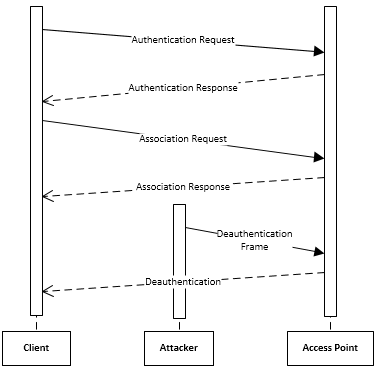
\includegraphics{research/attackvectors/figures/ddos.png}
\caption{Deauthentication DOS sequence.}
\end{figure}

The beauty of the deauthentication DOS is that it can be launched from relatively inexpensive hardware, as demonstrated with the Alfa, when paired with a good technical knowledge- especially when using a pre-support applications \cite{research:aircrack}. It should also be noted that this attack may not be started with malicious intent, as, for example, you have a network with a hidden SSID that users have discovered and hijacked, you can use this to deauthenticate all the stations to recover the network. On the more malicious side, this attack can be used to force users to connect to a spoofed access point after performing this attack, then chaining on a MITM attack. 

Chaining this attack with a spoofed access point, and then performing a MITM is an example of an advanced attack that could be performed on unknowing users in a public location. Utilizing beacon frames to start the chain of attack leaves security software that tracks spoofed MAC addresses completely useless. You can determine the MAC address of the real access point by monitoring beacon frames and taking the value set as the source address, then using it source in the deauthentication DOS, and then subsequently the spoofed access point setup.

\subsubsection*{Performing the Attack}
To gain a better understanding of this advanced attack I performed it on myself and documented the results. I set up my wireless router to broadcast an open network, laptop running BackTrack, tablet connected to the wireless network, and wireless adaptor in monitor mode.

\subsubsection*{Discovering the Access Point}
Although I knew the SSID and could get the MAC address of the access point I would be targeting, I wanted to perform it from the perspective of somebody that didn't, and needed to circumvent security software. In order to achieve this first step I decided to use the airomon-ng tool. This tool monitors beacon and probe request frames broadcast within range, and prints the MAC address of the source, and the SSID of the station. Figure \ref{ddos-1} shows the output of this application, and reveals the MAC address of the access point, ``Biggles'', I am targetting.

\begin{figure}[h!]
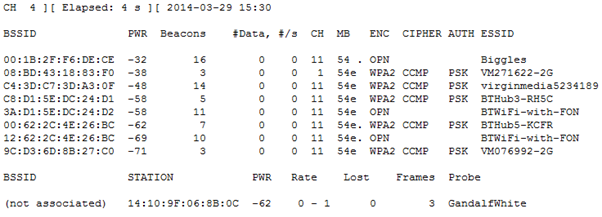
\includegraphics[width=\linewidth]{research/attackvectors/figures/ddos-1.png}
\caption{List of AP SSIDs in range of the wireless antenna.}
\label{ddos-1}
\end{figure}

\subsubsection*{Sending the Deauthentication Frame}
As the access point is transmitting on channel 11, I needed to either switch it to the same channel as the wireless adaptor monitor interface, or switch the monitor interface to channel 11. Again, as this was from the perspective of an attacker, I opted to switch the monitor interface channel as would be done in the field. After the channel change I could use aireplay-ng [8] to send a number of deauthentication frames with the spoofed MAC source and destination addresses, which is shown in figure \ref{ddos-3}.

\begin{figure}[h!]
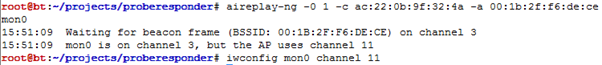
\includegraphics[width=\linewidth]{research/attackvectors/figures/ddos-2.png}
\caption{Changing the interface's channel.}
\end{figure}

\begin{figure}[h!]
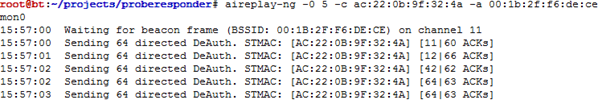
\includegraphics[width=\linewidth]{research/attackvectors/figures/ddos-3.png}
\caption{Sending the deauthentication frame.}
\label{ddos-3}
\end{figure}

\begin{figure}[h!]

\includegraphics[width=\linewidth]{research/attackvectors/figures/ddos-4.png}
\caption{Nexus 7 disassociating with the Netgear wireless router.}
\end{figure}

\subsubsection*{Introducing the Evil Twin}
To take this attack one step further toward the advanced chain of attacks, I created a fake access point that was making use of the Alfa wireless adaptor's ability to broadcast at a stronger signal than the access point. Figure \ref{ddos-5} shows the device connecting to the Evil Twin and leaving it open to any malicious intent I had.

\begin{figure}[h!]
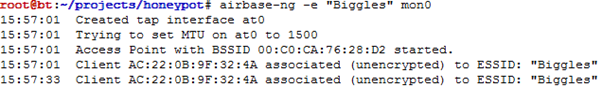
\includegraphics[width=\linewidth]{research/attackvectors/figures/ddos-5.png}
\caption{Station associating with the fake access point.}
\label{ddos-5}
\end{figure}